\section{Introduction}


A statement requiring citation \cite{Figueredo:2009dg}. Reference to Figure~\ref{fig:gallery}.\\

\begin{figure}[tb]
    \centering
    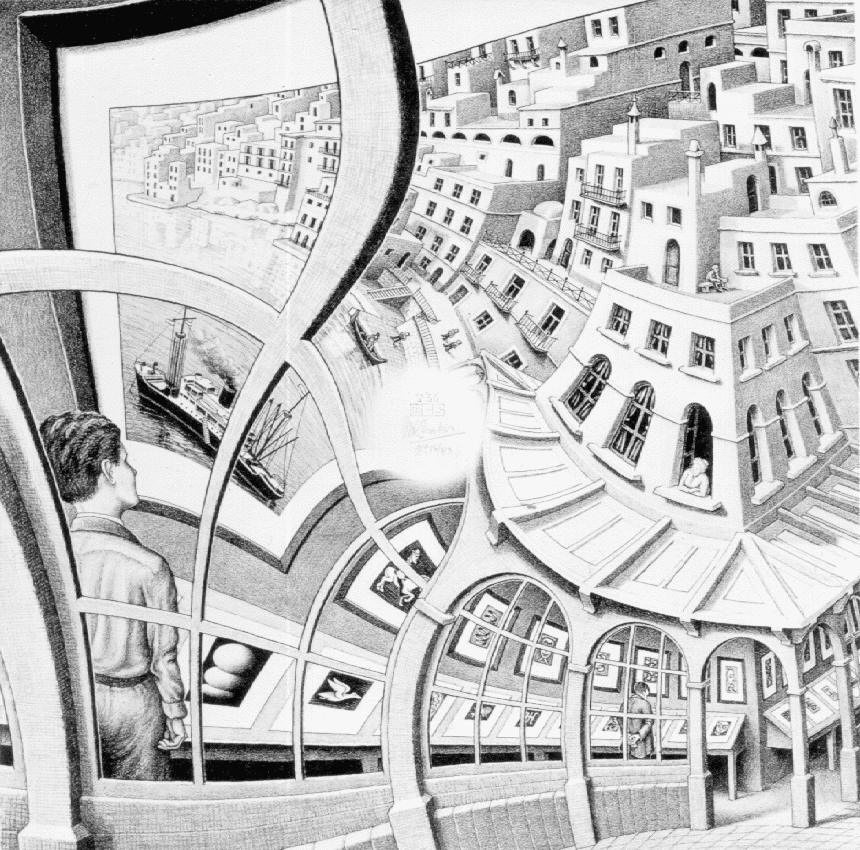
\includegraphics[width=0.5\columnwidth]{GalleriaStampe}
    \caption[An example of a floating figure]{An example of a floating figure (a reproduction from the \emph{Gallery of prints}, M.~Escher,\index{Escher, M.~C.} from \url{http://www.mcescher.com/}).} % The text in the square bracket is the caption for the list of figures while the text in the curly brackets is the figure caption
    \label{fig:gallery}
\end{figure}


\lipsum[1-3] % Dummy text

Some mathematics in the text: $\cos\pi=-1$ and $\alpha$.
